\begin{figure*}[t]
  \centering
  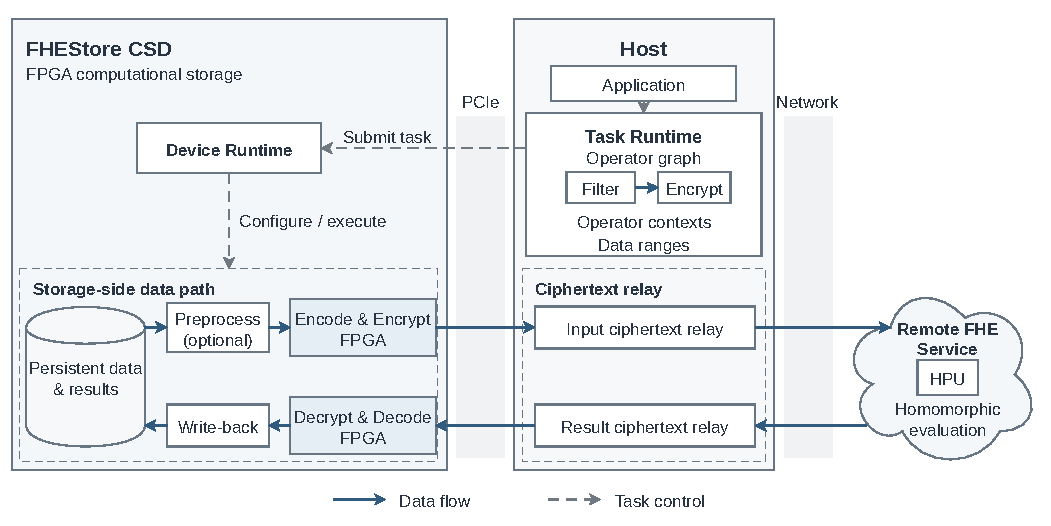
\includegraphics[width=\textwidth]{figures/fhestore-overview-v3/fhestore-overview.pdf}
  \caption{System overview of FHEStore. PCIe connects the host to the computational storage device and carries task submission and ciphertext handoffs. The host submits an operator graph, per-operator contexts, and data ranges to the device runtime, and relays input and result ciphertexts to and from the remote FHE service over the network. Solid arrows denote logical data flow; dashed arrows denote task control. Write-back is a system operation and may include host-assisted read--modify--write.}
  \Description{FHEStore computational storage connects to the host through PCIe, and the host connects to a remote FHE service through a network. The host application passes an operator graph, contexts, and data ranges to its task runtime, which submits the task over PCIe to the device runtime. The device runtime configures storage-side execution. Data from storage passes through optional preprocessing and FPGA encoding and encryption, over PCIe to the host input ciphertext relay, and over the network to the remote HPU service. Result ciphertexts return over the network to the host result relay and over PCIe to FPGA decryption and decoding, followed by write-back to storage.}
  \label{fig:fhestore-overview}
\end{figure*}
